\documentclass{article}
\usepackage[T1]{fontenc}
\usepackage[utf8]{inputenc}
\usepackage[polish]{babel}
\usepackage{amsmath}
\usepackage{amsfonts}
\usepackage{graphicx}
\usepackage{titlesec}
%{Informatyka stosowana 2024, I st., semestr VI}

\setcounter{secnumdepth}{4}

\titleformat{\paragraph}
{\normalfont\normalsize\bfseries}{\theparagraph}{1em}{}
\titlespacing*{\paragraph}
{0pt}{3.25ex plus 1ex minus .2ex}{1.5ex plus .2ex}


\author{
	{Amadeusz Sitnicki, 242524} \\
	{Adam Rosiak, 242511}\\
{Prowadzący: dr hab. inż. Bartłomiej Stasiak}
}

\title{Cyfrowe przetwarzanie sygnałów 2023/2024\\Projekt 1. Generacja sygnału i szumu}
\begin{document}
\maketitle
\section{Cel projektu}
Celem zadania jest stworzenie programu umożliwiającego generowanie sygnałów z zadaną częstotliwością próbkowania oraz implementacja podstawowych operacji pozwalających na generowanie nowego sygnału na podstawie 2 sygnałów bazowych. Dodatkowym celem jest stworzenie interfejsu użytkownika oraz wizualizacji w postaci wykresów wraz z podsumowaniem prezentującym podstawowe wartości  opisujące sygnał.

\section{Instrukcja korzystania z aplikacji}
Użytkownik korzysta z podwójnego menu pozwalającego na modyfikowanie parametrów wybranego typu sygnału - dostępnne menu dla sygnału A oraz menu dla sygnału B. Dla obu sygnałów użytkownik korzysta z odpowiedniego dla sygnału okna przewijanego zawierającego w pierwszej kolejności wykres wartości sygnału w zależności od czasu, a następnie histogram prezentujący dla ilu próbek sygnału, jego wartość znajdowała się w określonych przedziałach. Możliwe jest ustawienie z osobna dla obu sygnałów rozdzielczości histogramu przy użyciu suwaka. Poniżej suwaka znajduje się podsumowanie zawierające obliczoną średnią wartością sygnału, średnią wartością bezwzględną sygnału, średnią mocą sygnału, wariancją i wartością skuteczną sygnału. Rysunek \ref{fig:gui} przedstawia graficzny interfejs użytkownika wraz zawierający wspomniane w tej sekcji elementy interfejsu.

\begin{figure}[h!]
 \centering
 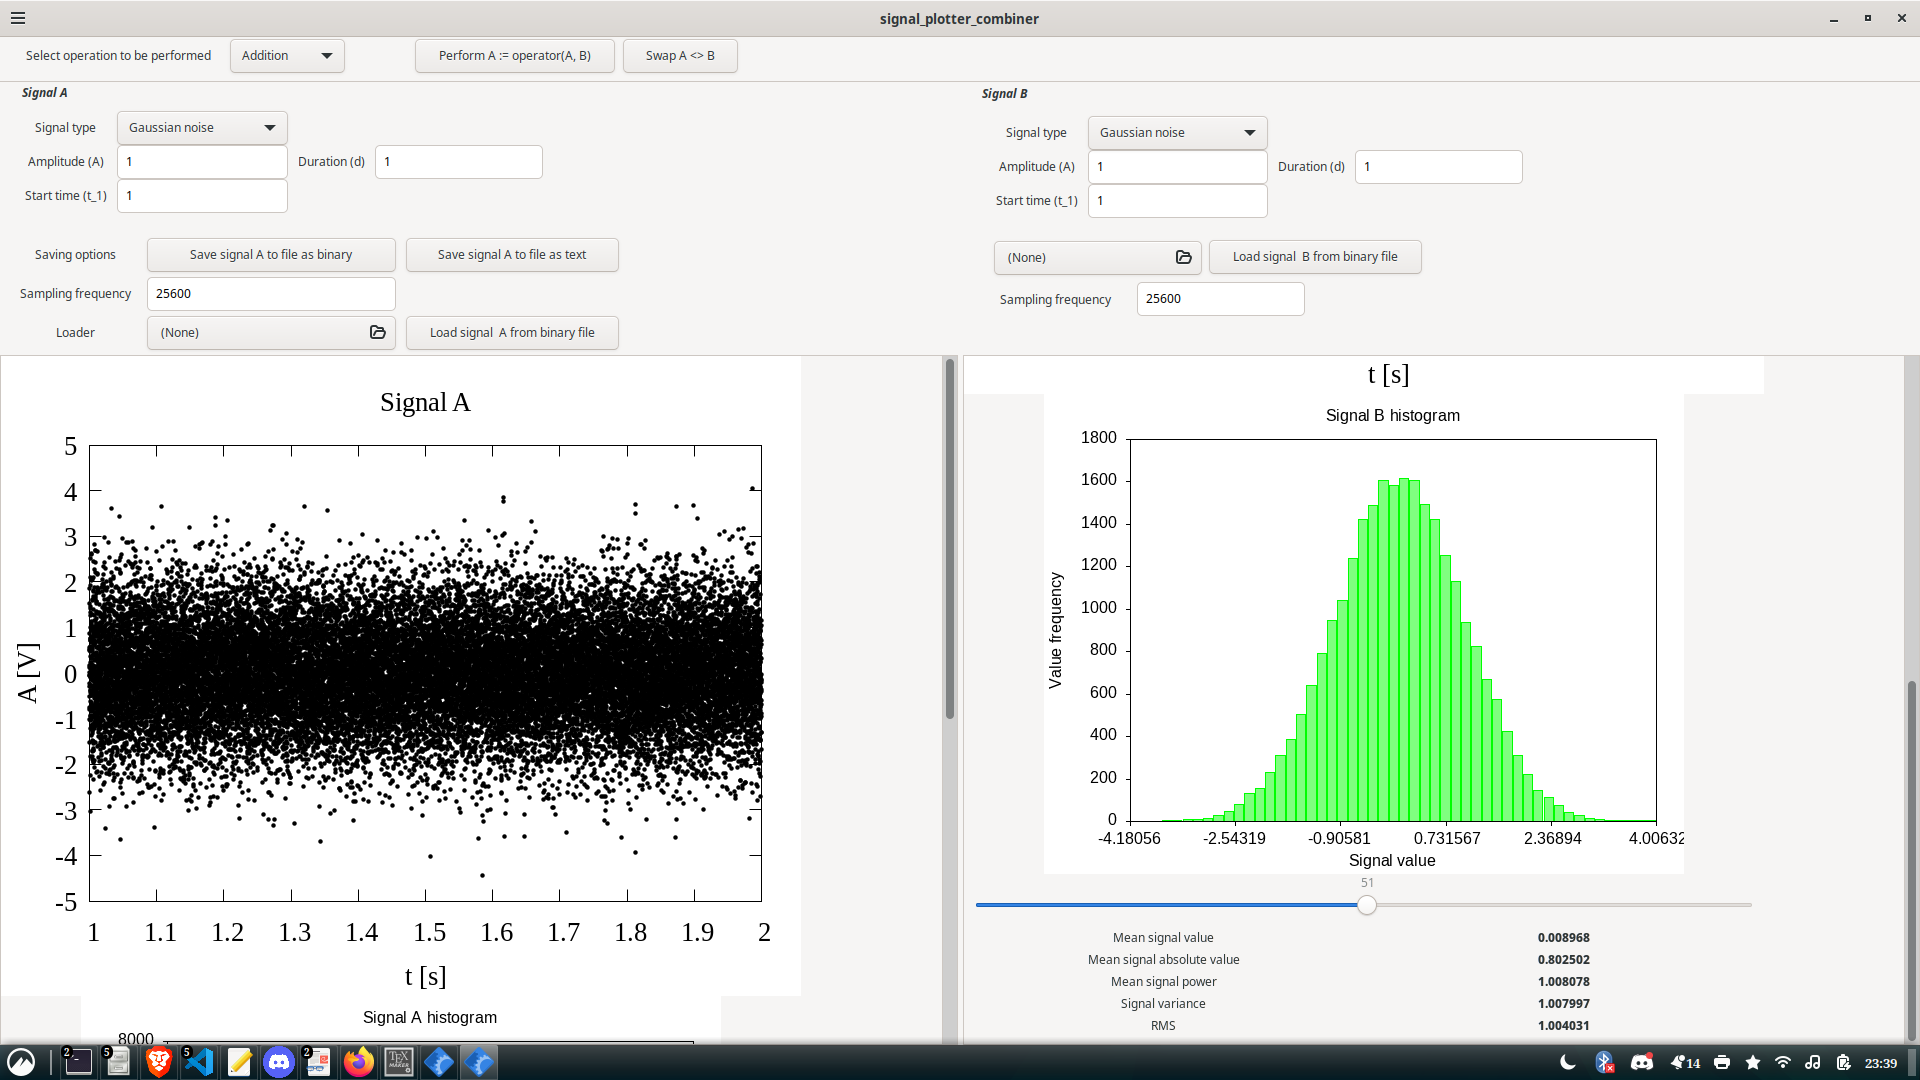
\includegraphics[width=14cm]{gui.png}
 \vspace{-0.3cm}
 \caption{Graficzny interfejs użytkownika programu}
 \label{fig:gui}
\end{figure}

\section{Opis implementacji oraz metod generowania danych do wykresów}
Aplikacja wykorzystuje otwartoźródłową bibliotekę graficznego interfejsu użytkownika GTK3 \cite{gtk3_link}.
Do implementacji wykorzystano język C wraz z kompilatorem GCC \cite{gcc_link} i systemem budowania Meson \cite{meson_link}, zapewniającym uproszczoną integrację z biblioteką GTK3.
W celu generowania wykresów, aplikacja posiada interfejs (\_gcall.h, gnuplot.h) dedykowany uruchamianiu procesu gnuplot - otwartoźródłowego narzędzia \cite{gnuplot_link} pozwalającego na tworzenie wykresów z wykorzystaniem skryptów w dedykowanym skryptowym języku gnuplot. Proces jest uruchamiany z przekazaniem parametrów zależnych od ustawień kontrolowanych przez użytkownika. Wykorzystano programowanie reaktywne - aplikacja reaguje na każdą zmianę parametrów sygnału i aktualizuje wykresy oraz podsumowania. Gnuplot pobiera dane generowane poprzez utworzenie przez aplikację pliku danych zawierającego specjalnie sformatowane dane sygnału i przekazanie jego ścieżki jako jeden z argumentów uruchomieniowych procesu gnuplot.
Przykład zbioru parametrów przekazanych do biblioteki znajduje się poniżej.
\begin{verbatim}
gnuplot -e "max=1." -e "min=-1." -e "n=10" -e "outfile='foo.png'"\ 
-e "infile='data.txt'" -e "plottitle='Signal A histogram'" script.plt
\end{verbatim}

Plik z danymi (odpowiadający plikowi data.txt w powyższym przykładzie) zawiera pary wartości (numer próbki, wartość próbki - oddzielone spacją) po jednej na linijkę.

Jak wspomniano, aplikacja umożliwia eksport i import sygnału z wykorzystaniem  specjalnego formatu zawartości pliku sygnału.
Format ten specyfikuje 24 bajty nagłówka, po których następują ośmiobajtowe  grupy odpowiadające wartościom sygnału (typ double) dla poszczególnych próbek.
Poniższe struktury języka C określają wspomniany format zawartości pliku sygnału (por. signal\_fio.h, signal.h)
\begin{verbatim}
typedef struct {
    double start_time;
    double sampling_frequency;
    uint64_t num_samples;
} signal_info_t;

typedef struct {
    union {
        signal_info_t info;
        uint64_t raw[3];
    } header;
    double* pData;
} real_signal_file_payload_t;
\end{verbatim}

Do całokształtu implementacji wykorzystano wzorzec MVC w celu odseparowania warstw modelu, widoku i kontrolera widoku. Warstwa widoku została zaimplementowana z użyciem pliku XML generowanego przez otwartoźródłowe narzędzie Glade, dedykowane projektowaniu graficznych interfejsów użytkownika dla biblioteki GTK3. 
W celu generowania wartości losowej o standardowym rozkładzie normalnym, użyto metody Marsaglia \cite{marsaglia_method_link}, której przykładową, uproszczoną implementację przedstawiono poniżej.
\begin{verbatim}
/**
 * Uses Marsaglia polar method and rand() to generate a standard-normally 
 distributed pseudo-random floating-point value
 * 
*/
double __standard_gaussian_rand() {
    double x; double y; 
    double s;
    do {
        x = -1.0 + 2 * ((double)rand()) / (double)RAND_MAX;
        y = -1.0 + 2 * ((double)rand()) / (double)RAND_MAX;
        s = x*x + y*y;
    } while (s >= 1.0);
    return x * sqrt(-2.0 * log(s) / s);
}
\end{verbatim}

\newpage
\section{Przykłady i wnioski z analizy działania programu}
\subsection{Przykład A - sygnał sinusoidalny}
\begin{figure}[h!]
 \centering
 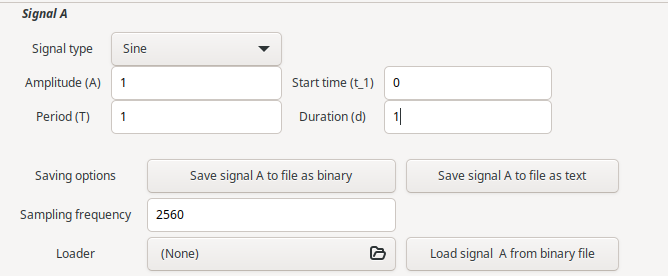
\includegraphics[width=14cm]{sine_config.png}
 \vspace{-0.3cm}
 \caption{Konfiguracja dla przykładowego sygnału sinusoidalnego}
 \label{fig:sine_config}
\end{figure}
\newpage
\begin{figure}[h!]
 \centering
 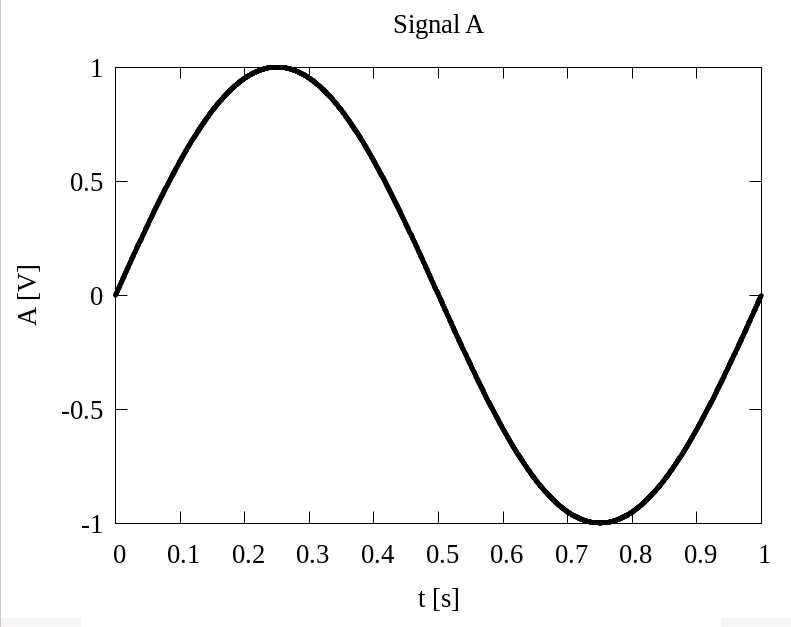
\includegraphics[width=14cm]{sine_plot.png}
 \vspace{-0.3cm}
 \caption{Wykres wartości sygnału sinusoidalnego}
 \label{fig:sine_plot}
\end{figure}
\newpage
\begin{figure}[h!]
 \centering
 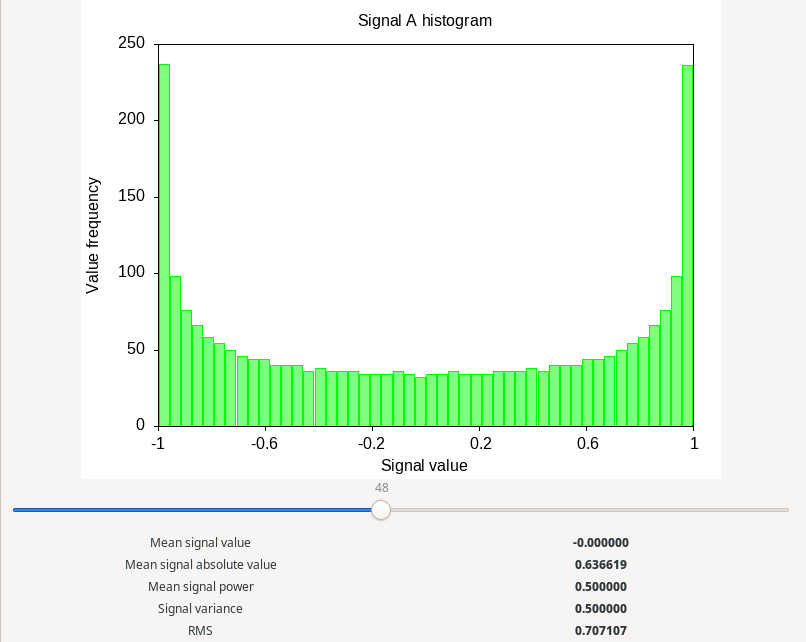
\includegraphics[width=14cm]{sine_histosum.png}
 \vspace{-0.3cm}
 \caption{Histogram i wartości agregatów dla sygnału sinusoidalnego}
 \label{fig:sine_histosum}
\end{figure}
\newpage
\subsection{Wniosek do przykładu A}
Skrajne wartości sygnału występują wśród próbek sygnału częściej, jest to spowodowane faktem, że w pobliżu ekstremów, funkcja sinus zmienia się wolniej, zatem jest więcej próbek przypadających na zadany przedział wartości. Dodatkowo warto zwrócić uwagę, że średnia wartość sygnału sinusoidalnego na przedziale o długości będącej wielokrotnością długości okresu, jest równa 0. Wariancja wartości sygnału oraz średnia moc sygnału mają wartość 0,50.
Wartość skuteczna sygnału jest odwrotnością pierwiastka kwadratowego liczby 2.
\subsection{Przykład B - szum gaussowski}
\begin{figure}[h!]
 \centering
 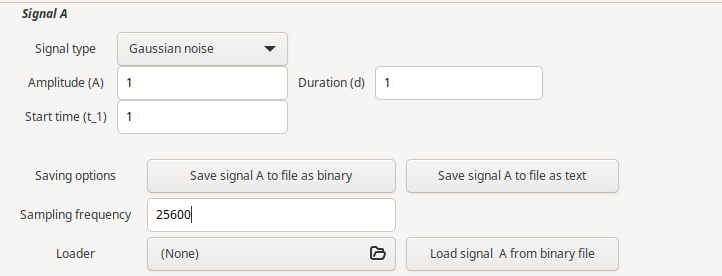
\includegraphics[width=14cm]{gauss_config.png}
 \vspace{-0.3cm}
 \caption{Konfiguracja dla standardowego szumu gaussowskiego}
 \label{fig:gauss_config}
\end{figure}
\newpage
\begin{figure}[h!]
 \centering
 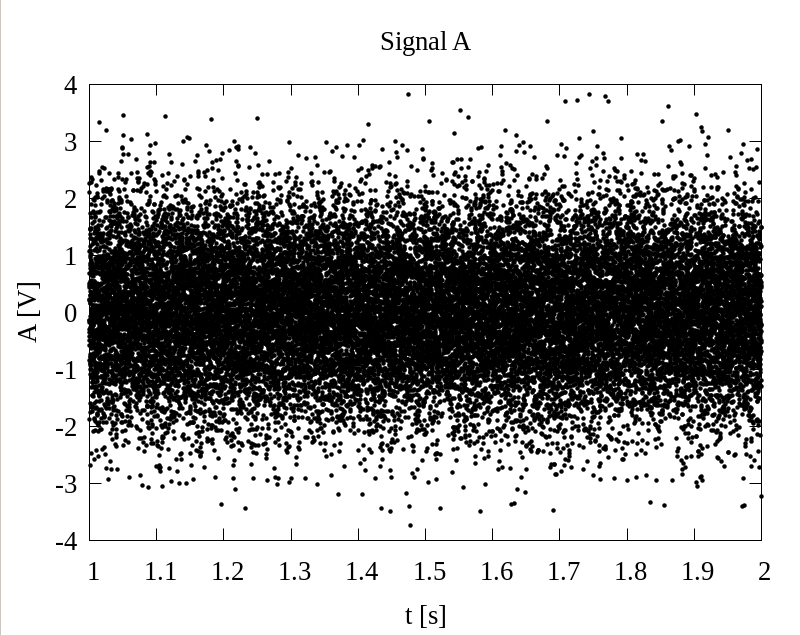
\includegraphics[width=14cm]{gauss_plot.png}
 \vspace{-0.3cm}
 \caption{Wykres wartości standardowego szumu gaussowskiego}
 \label{fig:gauss_plot}
\end{figure}
\newpage
\begin{figure}[h!]
 \centering
 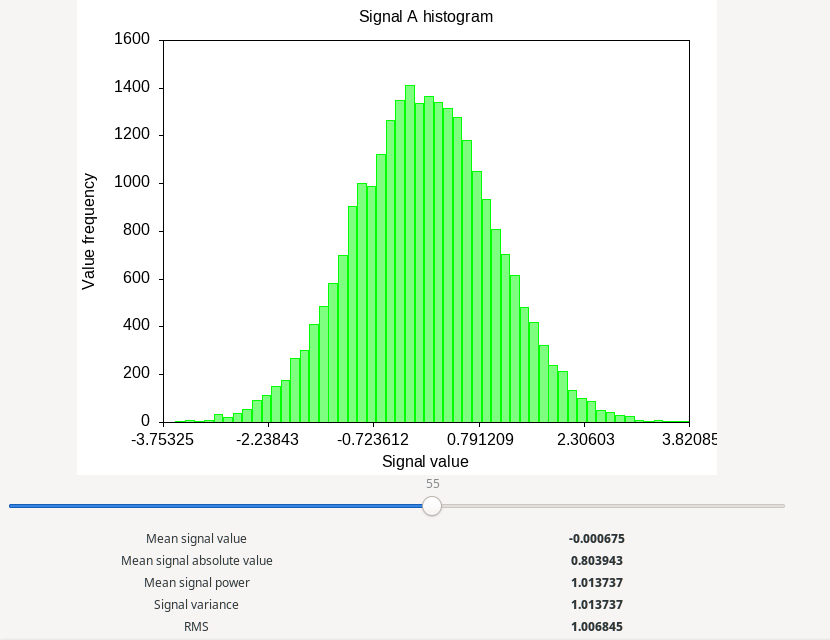
\includegraphics[width=14cm]{gauss_histosum.png}
 \vspace{-0.3cm}
 \caption{Histogram i wartości agregatów dla standardowego szumu gaussowskiego}
 \label{fig:gauss_histosum}
\end{figure}
\newpage
\subsection{Wniosek do przykładu B}
Metoda polarna Marsaglia jest skutecznym sposobem na otrzymanie przybliżonego standardowego rozkładu normalnego pseudo-losowego wartości zmiennoprzecinkowych. Wartość skuteczna szumu jest bliska 1. Zgodnie z definicją użytego rozkładu, wartość oczekiwana dla sygnału jest bliska 0, a wariancja wynosi  w przybiżeniu 1.
\subsection{Przykład C - kombinacja sygnałów z użyciem prostej operacji dodawania}
\begin{figure}[h!]
 \centering
 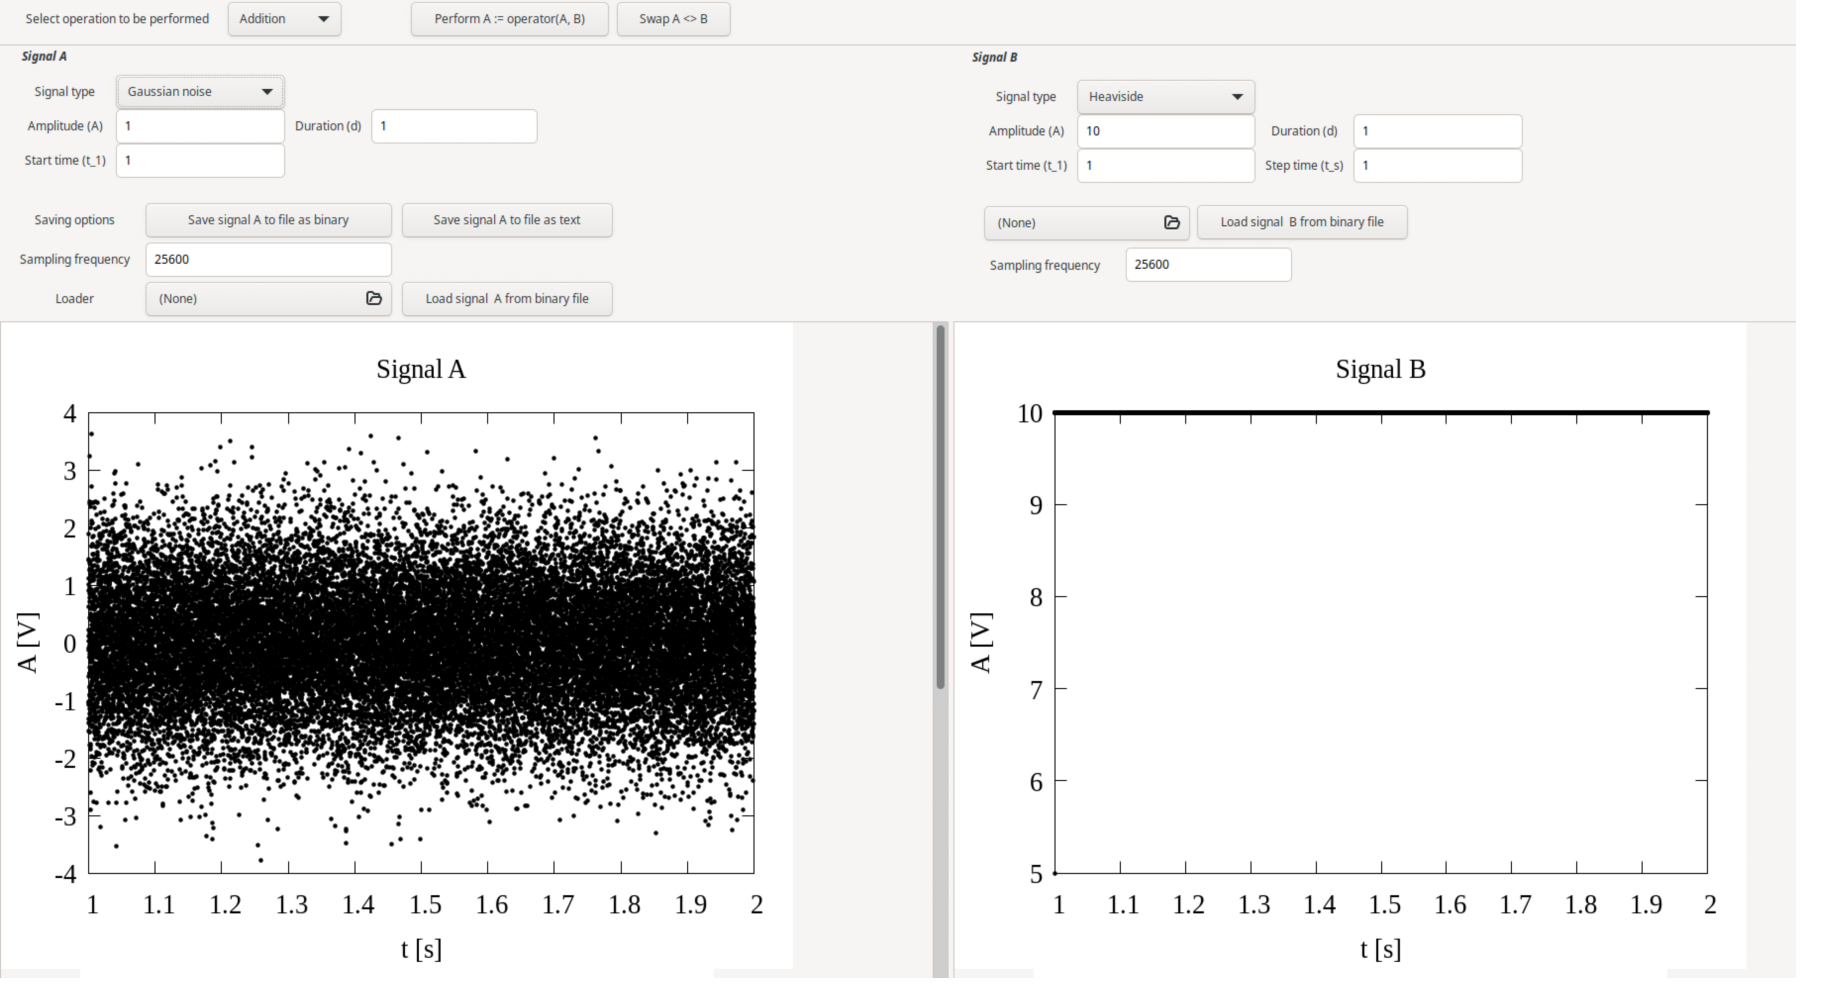
\includegraphics[width=14cm]{add_plotconfig.png}
 \vspace{-0.3cm}
 \caption{Konfiguracja dla dodawania sygnału o stałej wartości 10 do szumu gaussowskiego}
 \label{fig:add_plotconfig}
\end{figure}
\newpage
\begin{figure}[h!]
 \centering
 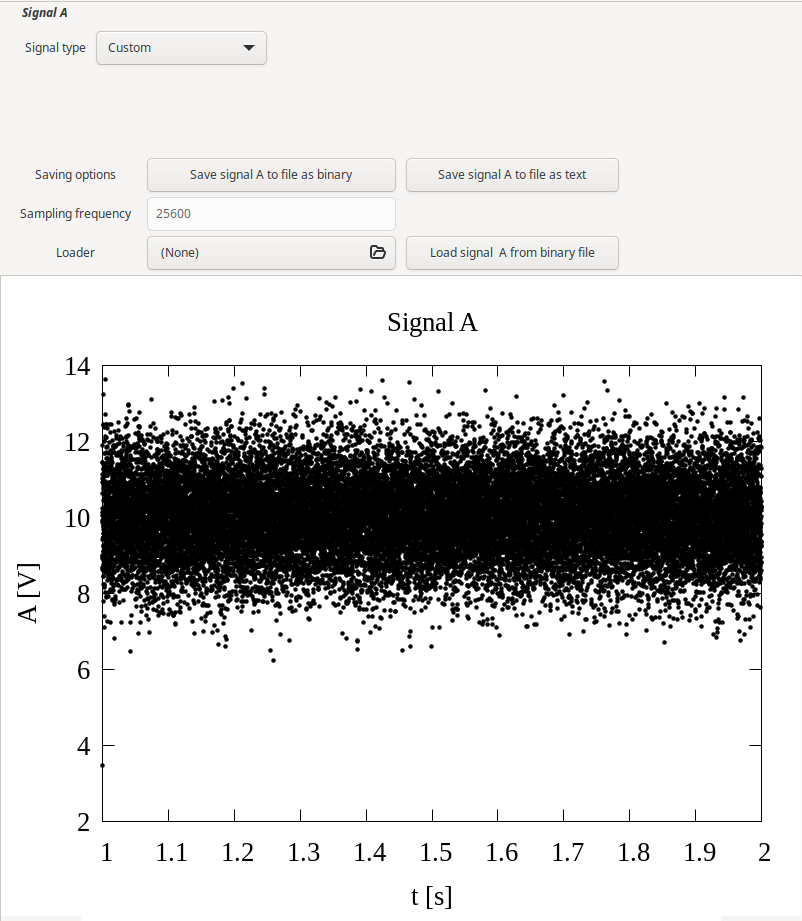
\includegraphics[width=14cm]{shifted_gauss.png}
 \vspace{-0.3cm}
 \caption{Wykres wartości sygnału wynikowego operacji dodawania - przesunięty standardowy szum gaussowski}
 \label{fig:shifted_gauss}
\end{figure}
\newpage
\begin{figure}[h!]
 \centering
 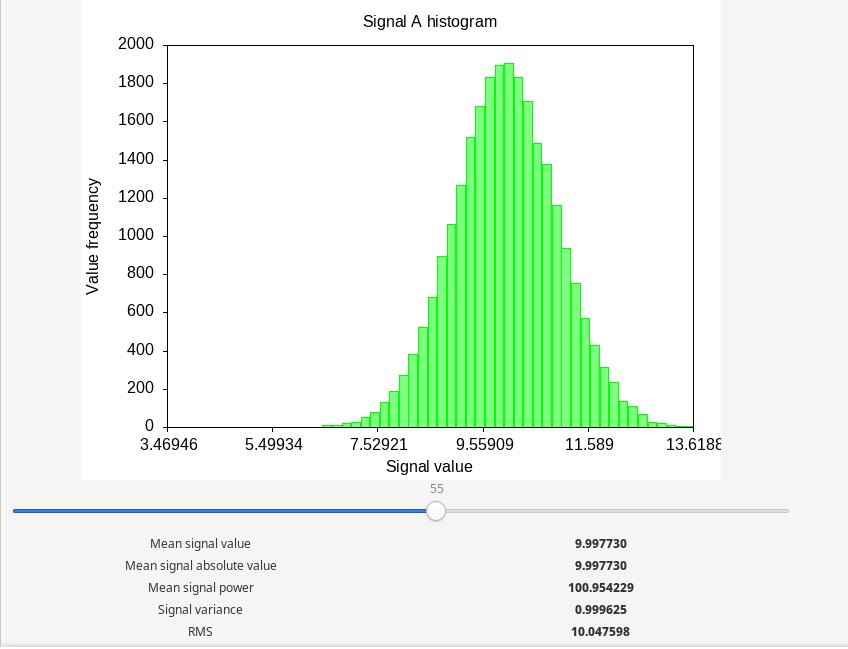
\includegraphics[width=14cm]{shifted_gauss_hist.png}
 \vspace{-0.3cm}
 \caption{Histogram dla sygnału wynikowego operacji dodawania - przesunięty standardowy szum gaussowski}
 \label{fig:shifted_gauss_hist}
\end{figure}
\newpage
\subsection{Wniosek do przykładu C}
Dodanie dodatniego sygnału stałego do szumu gaussowskiego powoduje przesunięcie wykresu na histogramie w prawo - operacja dodawania zachodzi pomyślnie. Zaobserwować można ustalenie się wartości skutecznej oraz średniej wartości sygnału i średniej absolutnej wartości sygnału na poziomie o 10 wyższym niż w przypadku standardowego rozkładu gaussowskiego bez przesunięcia - liniowa zmiana względem przesunięcia wartości sygnału. Wariancja sygnału nie uległa zmianie względem szumu bez przesunięcia, zaś średnia moc wzrosła o kwadrat przesunięcia wartości szumu.

\begin{thebibliography}{0}
\bibitem{gtk3_link} GTK3, strona projektu, https://docs.gtk.org/gtk3/
\bibitem{gcc_link} GCC, strona projektu, https://gcc.gnu.org/  
\bibitem{meson_link} Meson Build, strona projektu, https://mesonbuild.com/
\bibitem{gnuplot_link} Gnuplot, strona główna projektu, http://www.gnuplot.info/
\bibitem{marsaglia_method_link} Marsaglia G., Bray T.A. (1964), A Convenient Method for Generating Normal Variables
\end{thebibliography}

Literatura zawiera wyłącznie źródła recenzowane i/lub o potwierdzonej wiarygodności,
możliwe do weryfikacji i cytowane w sprawozdaniu. 
\end{document}